\section{強度を考慮し再設計したロボットの解析}\label{ux5f37ux5ea6ux3092ux8003ux616eux3057ux518dux8a2dux8a08ux3057ux305fux30edux30dcux30c3ux30c8ux306eux89e3ux6790}

ここでは,強度をあげるために再設計したロボットアームの解析を行う.

解析の手順は,基準となるロボットの解析をした時及び手先加速度を上げるために再設計したロボットについて解析した時と同じである.

\subsection{強度を考慮し再設計したロボットの構造解析}\label{ux5f37ux5ea6ux3092ux8003ux616eux3057ux518dux8a2dux8a08ux3057ux305fux30edux30dcux30c3ux30c8ux306eux69cbux9020ux89e3ux6790}

強度を考慮して再設計したロボットの構造解析を行う.

SolidEdgeを使って求めたリンクアームの体積,質量,慣性モーメントに加え,材質と密度をまとめて記載したものが表\ref{strong-robot-data}である.

\begin{table}[htb]
\caption[]{リンクアームの各値}
  \begin{center}
    \begin{tabular}{|c|c|} \hline
      材質 & アルミニウム1060 \\ \hline
      密度 [$\rm kg/m^3$]& 2712.0 \\ \hline
      体積[$\rm m^3$] & 0.20503 \\ \hline
      質量[kg] & 556.052 \\ \hline
      慣性モーメント & 765.744 [$\rm kg m^2$] \\ \hline
    \end{tabular}
    \label{strong-robot-data}
  \end{center}
\end{table}

まず,慣性モーメントについて考える.

基準となるロボットとは異なり,形状が複雑となり,慣性モーメントを求めるのが複雑であるので,慣性モーメントの理論値とシミュレーションによって求めた慣性モーメントの値の大小関係が一致しているかという点でシミュレーション結果の妥当性を考える.

今回の手先加速度をあげるために再設計したロボットのアームについて,重心軸周りの慣性モーメント\(I_G\)は\(265.419[\rm kgm^2]\)となった.

ゆえに,軸間距離\(d=0.954[\rm m]\),重心周りの慣性モーメント\(I_G=265.419[\rm kgm^2]\)及び質量\(M=556.052[\rm kg]\)を使い,平行軸の定理より慣性モーメントを求めると式\ref{solveStrongKansei}となる.

\begin{eqnarray}
  I &=& I_G+d^2M \nonumber \\
    &=& 265.419 + 0.954^{2} 556.052 \nonumber \\
    &=& 771.491
  \label{solveStrongKansei}
\end{eqnarray}

となるので,平行軸の定理を用いて求めた慣性モーメントの値は771.491\([\rm kgm^2]\),シミュレーションで得た慣性モーメントの値は765.744\([\rm kgm^2]\)とほぼ一致しているため,今回のシミュレーション結果は正しいといえる.

また,強度をあげるために再設計したロボットは,基準ロボットの根元部分を分厚くして補強したものであるので,慣性モーメント及び質量は大きくなっていることが予想される.

基準ロボットと今回強度をあげるために再設計したロボットの体積,質量及び慣性モーメントの値を比較したのが表\ref{compare-basic-strong-mass}である.

\begin{table}[htb]
\caption[]{リンクアームの各値}
  \begin{center}
    \begin{tabular}{|c|c|c|} \hline
      項目 & 基準アーム & 強度を重視して再設計したアーム \\ \hline \hline
      体積[$\rm m^3$] & 0.17915 &0.20503 \\ \hline
      質量[kg] & 485.832 & 556.052 \\ \hline
      慣性モーメント[$\rm kg m^2$] & 751.9 & 765.744 \\ \hline
    \end{tabular}
    \label{compare-basic-strong-mass}
  \end{center}
\end{table}

表\ref{compare-basic-strong-mass}を見て分かるように,再設計後は体積,質量,慣性モーメントの全てが大きくなっているため,SolidEdgeの解析結果は正しいことが分かる.

今回,質量の上昇量に対して慣性モーメントはあまり大きく変動しなかった.

ロボットアームの慣性モーメント\(I\)は,微小部分の慣性モーメント\(dI\)をアーム全体で積分したものなので,式\ref{bisyo-kansei}と書くことが出来る.

\begin{eqnarray}
  I &=& \int dI
  \label{bisyo-kansei}
\end{eqnarray}

ここで,この物体の微小部分が作る慣性モーメント\(dI\)はその微小部分の回転中心からの距離\(r\)とその部分の微小質量\(dm\)を使って,式\ref{bisyo}と書ける.

\begin{eqnarray}
  dI &=& r^2 dm 
  \label{bisyo}
\end{eqnarray}

式\ref{bisyo}からわかるように,回転中心に近い場所の質量を大きくした場合,質量の増加量に対して慣性モーメントの増加量は小さくなり,回転中心から遠い場所の質量を重くした場合,質量の増加量に対して慣性モーメントの増加量は大きくなる.

今回,回転中心に近い場所を補強し,質量を大きくしたため,理論的には質量の上昇量に対して慣性モーメントはあまり大きく変動しないという結果が得られるはずであり,これも今回の解析結果と一致する.

\subsubsection{応力の解析}\label{ux5fdcux529bux306eux89e3ux6790}

次に,応力の解析及びその解析結果の検証を行っていく.
手先加速度をあげるために再設計したロボットのアームの応力図を図\ref{strong-ouryoku}に示す.

\begin{figure}[htbp]
  \begin{center}
    \begin{tabular}{c}
      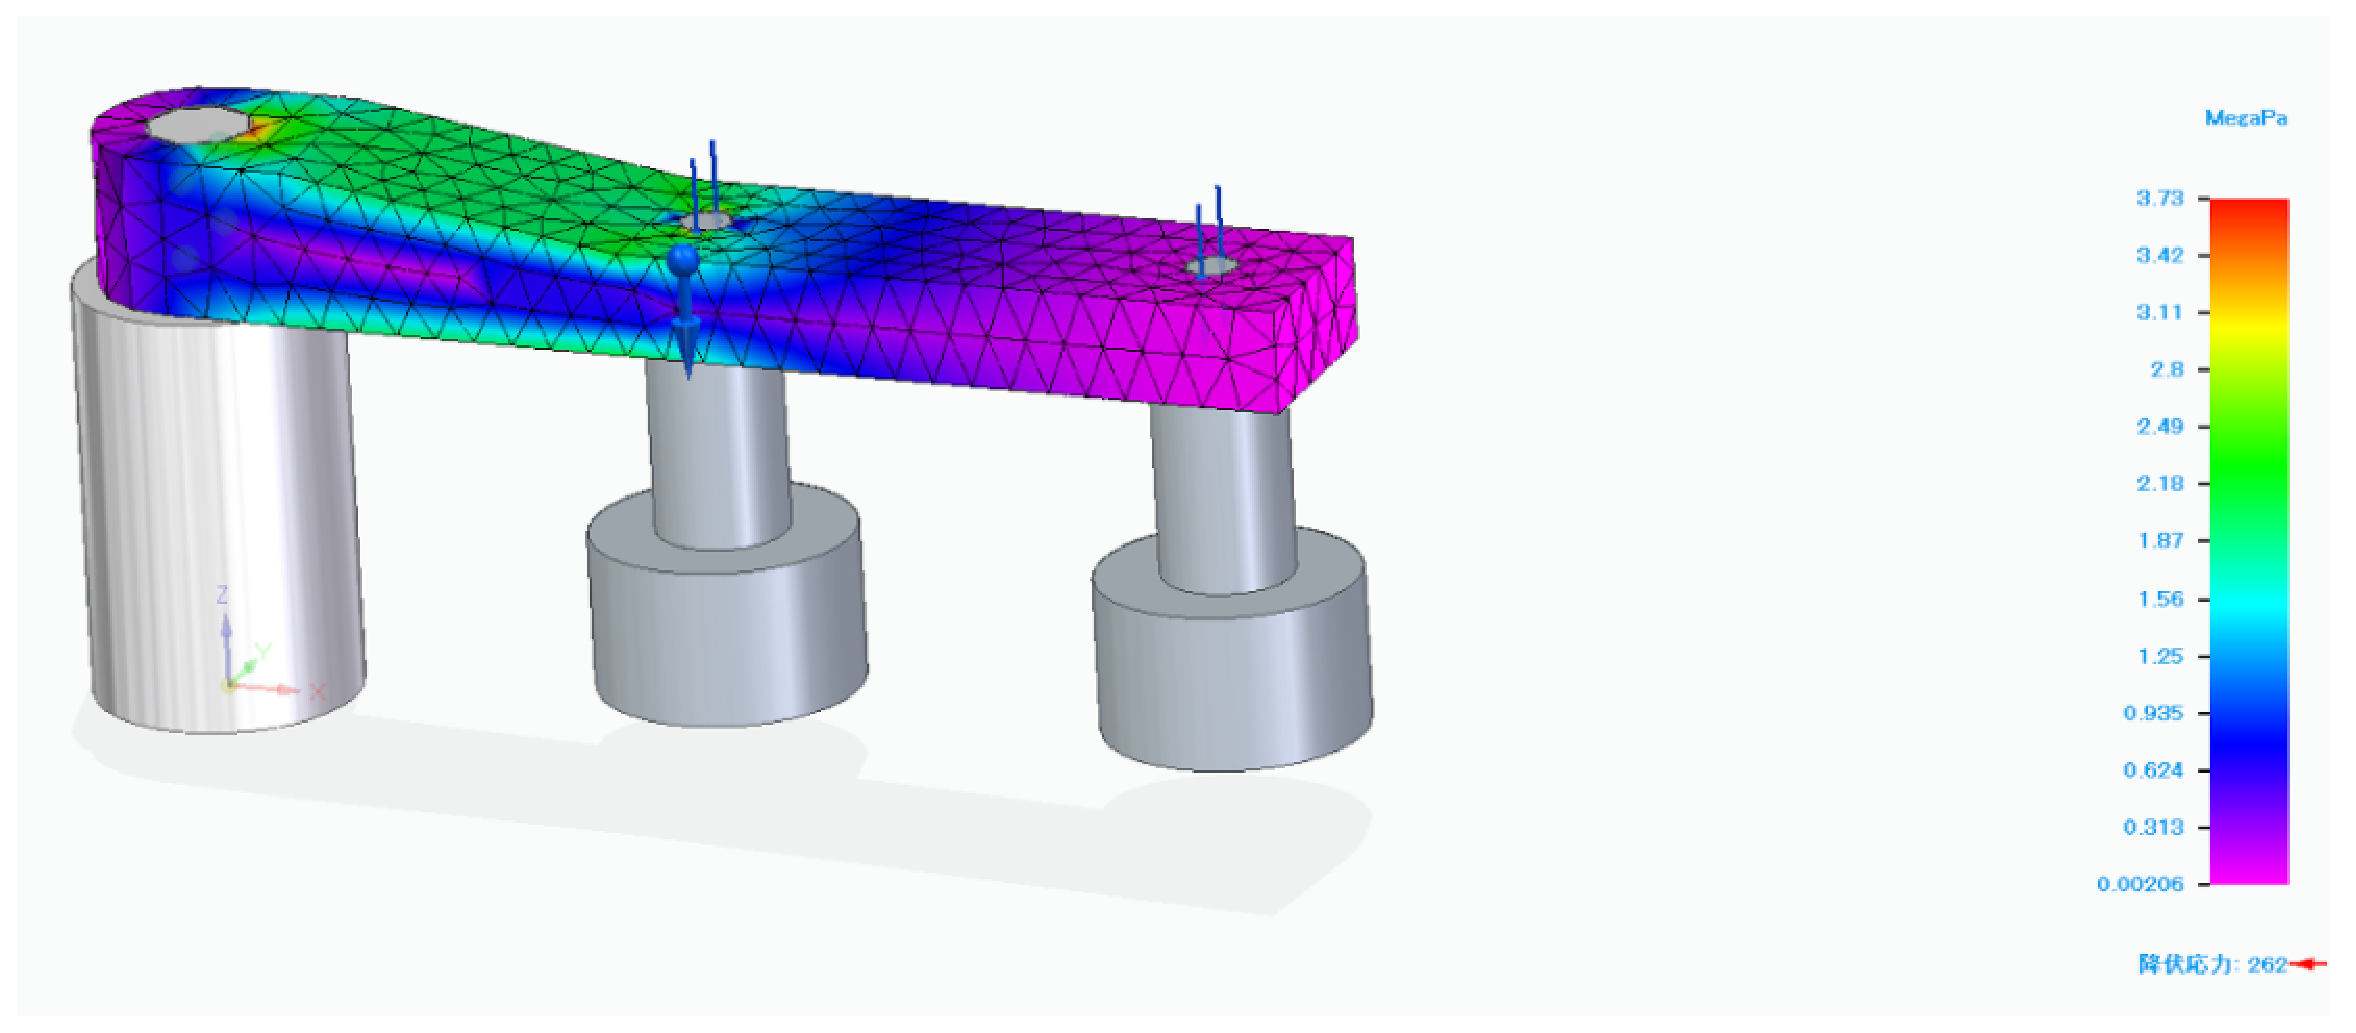
\includegraphics[height=6.5cm]{img/eps/strong-ouryoku.eps}
    \end{tabular}
    \caption{強度を重視したロボットの構造解析の応力図}
    \label{strong-ouryoku}
  \end{center}
\end{figure}

この時,図\ref{strong-ouryoku-result}に示す結果がSolid
Edgeより出力された.

\begin{figure}[htbp]
  \begin{center}
    \begin{tabular}{c}
      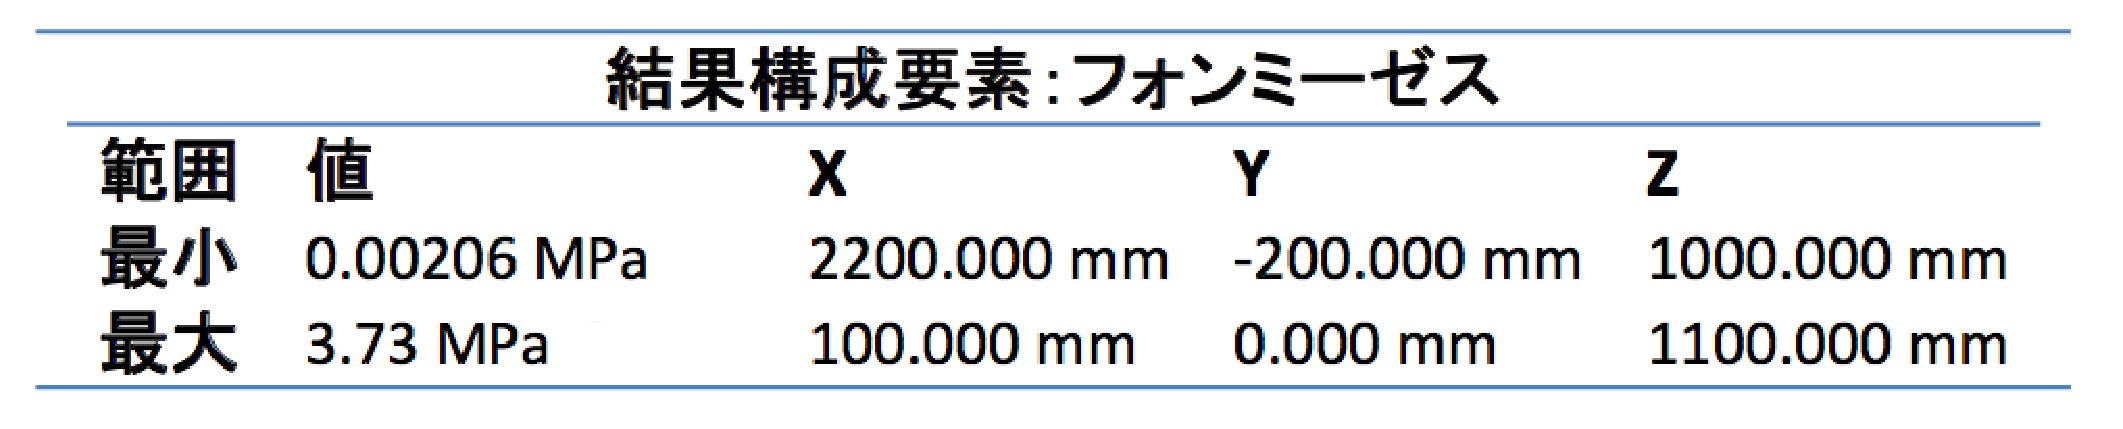
\includegraphics[height=2.5cm]{img/eps/strong-ouryoku-result.eps}
    \end{tabular}
    \caption{強度を重視したロボットの応力解析結果}
    \label{strong-ouryoku-result}
  \end{center}
\end{figure}

基準となるロボットアームに比べて今回のロボットは形状が複雑であるので,このシミュレーション結果の妥当性を,解析解の大小関係によって評価する.

基準となるロボットアームの根元部分に大きな応力がかかることがわかったので,今回は強度を高めるためにアーム根元部分の断面積を増やした.

よって,今回の強度を高めるために再設計したロボットアームは,応力が基準となるロボットアームより小さくなっている必要がある.

基準ロボットの最大応力は6.81{[}MPa{]}であり,今回強度を重視して再設計の最大応力は3.73{[}Mpa{]}であったため,シミュレーション結果は正しいと考えられる.

許容応力は27.6{[}MPa{]}であるので,安全率は式\ref{strong-anzen}より,7.39となる.

\begin{eqnarray}
  安全率 &=& \frac{許容応力}{最大応力} \nonumber \\ &=& 7.39
  \label{strong-anzen}
\end{eqnarray}

\subsubsection{変位の解析}\label{ux5909ux4f4dux306eux89e3ux6790}

次に,重力及び荷重によってかかる変位について解析する.

Solid
Edgeのシミュレーション機能を用いて変位を解析した所,変位分布は図\ref{strong-heni}となった.

\begin{figure}[htbp]
  \begin{center}
    \begin{tabular}{c}
      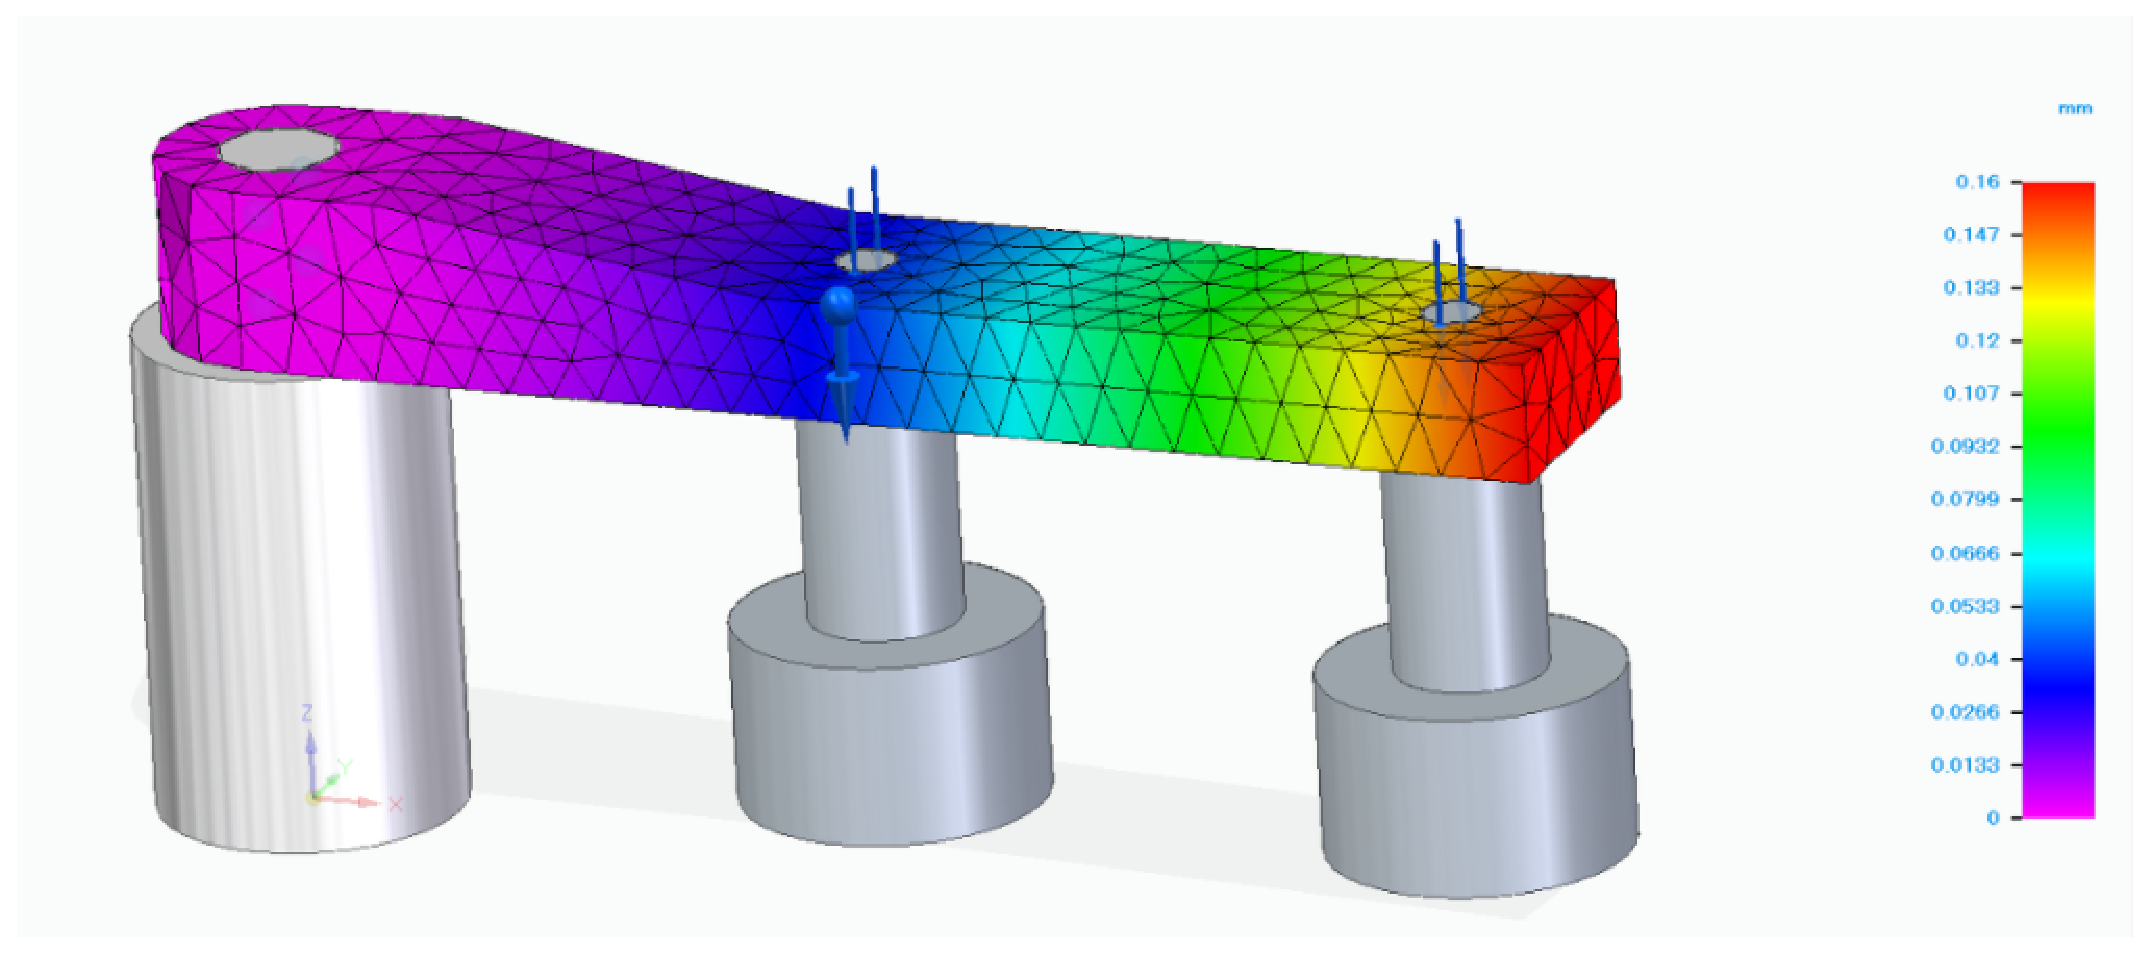
\includegraphics[height=6.5cm]{img/eps/strong-heni.eps}
    \end{tabular}
    \caption{強度を上げるために再設計したロボットの変位分布}
    \label{strong-heni}
  \end{center}
\end{figure}

この時,図\ref{strong-heni-result}に示す変位結果がSolid
Edgeより出力された.

\begin{figure}[htbp]
  \begin{center}
    \begin{tabular}{c}
      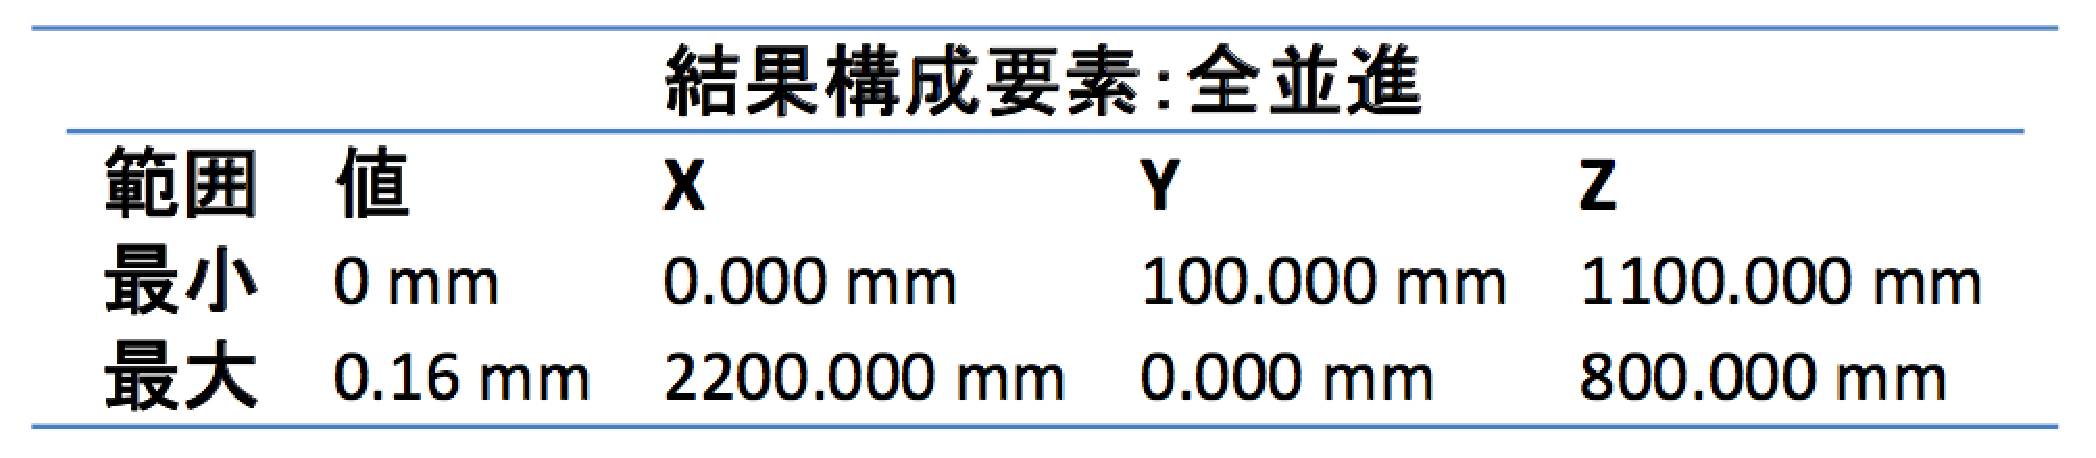
\includegraphics[height=2.5cm]{img/eps/strong-heni-result.eps}
    \end{tabular}
    \caption{強度を上げるために再設計したロボットの変位解析結果}
    \label{strong-heni-result}
  \end{center}
\end{figure}

強度を上げるために再設計したロボットは,根本の断面積が大きく,たわみにくい.よってたわみ角が小さくなるので,理論的には基準となるロボットアームよりたわみ量が小さくなるはずである.

実際,基準となるロボットアームの変位は0.541{[}mm{]}であり,今回強度を重視し再設計したアームの変位は0.16{[}mm{]}となった.

よって,シミュレーション結果は正しいと考えられる.

\subsection{強度をあげるために再設計したロボットの機構解析}\label{ux5f37ux5ea6ux3092ux3042ux3052ux308bux305fux3081ux306bux518dux8a2dux8a08ux3057ux305fux30edux30dcux30c3ux30c8ux306eux6a5fux69cbux89e3ux6790}

ロボットアームに対して,基準座標系\(\Sigma_0\),リンク座標系\(\Sigma_1\),及び手先座標系\(\Sigma_E\)を記述したのが図\ref{strong-tesaki}である.

\begin{figure}[htbp]
  \begin{center}
    \begin{tabular}{c}
      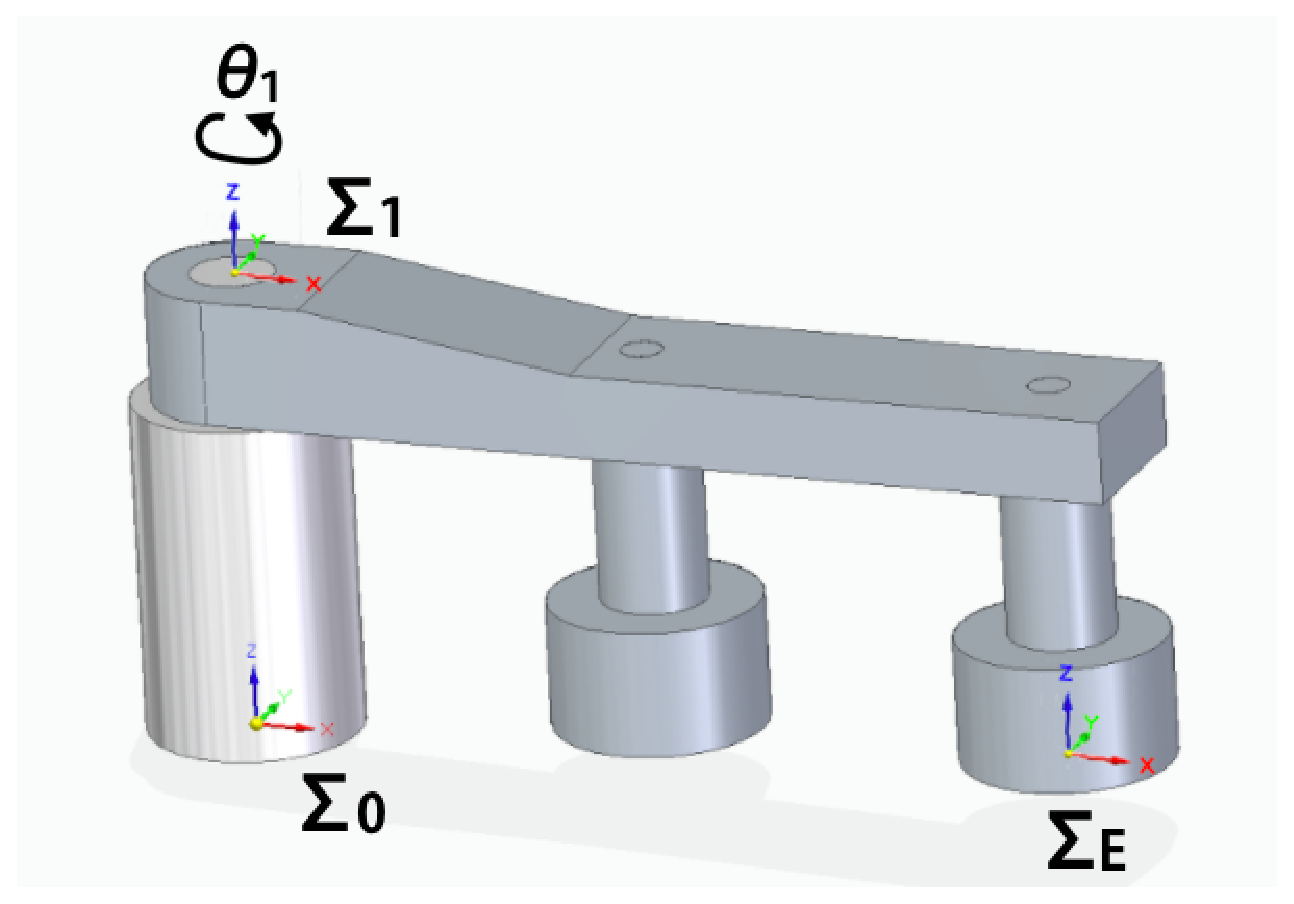
\includegraphics[height=5.5cm]{img/eps/strong-dh.eps}
    \end{tabular}
    \caption{強度を考慮し再設計したロボットの各種座標系}
    \label{strong-tesaki}
  \end{center}
\end{figure}

このロボットアームのリンクパラメータをDH記法を用いて書くと表\ref{strong-dh-link}となる.
今回,手先としてアーム先端のブレード部分を選んだ.

\begin{table}[htb]
\caption[]{リンクパラメータ}
  \begin{center}
    \begin{tabular}{|c|c|c|c|c|} \hline
      $i$ & $a_{i-1}$ & $\alpha_{i-1}$ & $d_i$ & $\theta_i$\\ \hline \hline
      1 & 0 & 0 & 1100[mm] & ($\theta_1$) \\ \hline
      2 & 2000[mm] & 0 & -900[mm] & 0 \\ \hline
    \end{tabular}
    \label{strong-dh-link}
  \end{center}
\end{table}

次に,関節角度の理論解及びシミュレーション結果を比較する.

SimXpertを使用して,今回作成したアームロボットの関節回転角度を求めた結果を図\ref{strong-kaiten}に示す.

\begin{figure}[htbp]
  \begin{center}
    \begin{tabular}{c}
      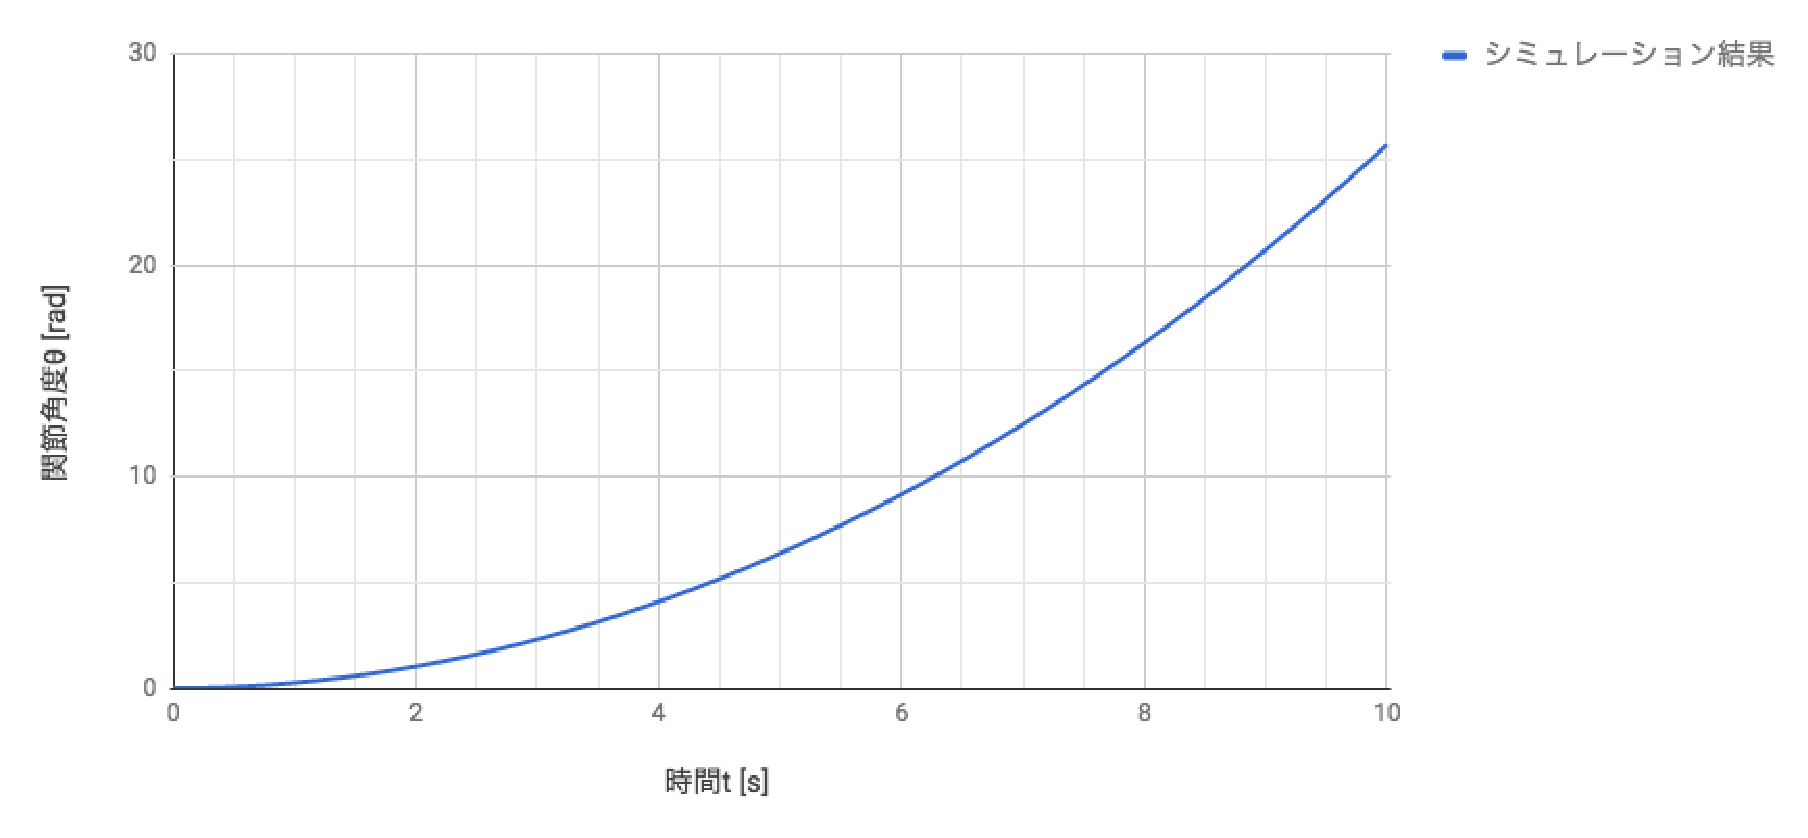
\includegraphics[height=5.0cm]{img/eps/strong-kaiten2.eps}
    \end{tabular}
    \caption{強度をあげるために再設計したロボットのアームの関節回転角}
    \label{strong-kaiten}
  \end{center}
\end{figure}

この関節角度のシミュレーション結果を最小二乗法を用いて2次の多項式近似を行うと,式\ref{strong-niji-kinji}を得ることが出来る.

\begin{eqnarray}
  \frac{d\theta}{dt} &=& 0.259t^2+0.029x-0.0037 \nonumber \\
  &\approx& 0.259t^2
  \label{strong-niji-kinji}
\end{eqnarray}

式\ref{kaiten-houteisiki}で示した回転の運動方程式に,関節駆動トルク\(\tau=393\),そして慣性モーメント\(I=765.744\)を代入すると,式\ref{strong-kaiten-houteisiki-calc}となる.

\begin{eqnarray}
  393 &=& 765.744 \frac{d^2 \theta}{d t^2}
  \label{strong-kaiten-houteisiki-calc}
\end{eqnarray}

式\ref{strong-kaiten-houteisiki-calc}は,時間に関する2階微分であるので,速度及び角度の初期値を0として両辺時間で2度積分することで微分方程式を解くと,式\ref{strong-deg}の角度の関数を得る.

\begin{eqnarray}
  \theta = 0.2566t^2
  \label{strong-deg}
\end{eqnarray}

SimXpertのシミュレーション結果の式\ref{strong-niji-kinji}と式\ref{strong-deg}は完全に一致していると言って良い.

先ほどSimXpertで得られたシミュレーションの結果と,式\ref{strong-deg}で求めた\(\theta\)の理論解を比較したのが図\ref{strong-compare}であり,2つのグラフは完全に一致している.

\begin{figure}[htbp]
  \begin{center}
    \begin{tabular}{c}
      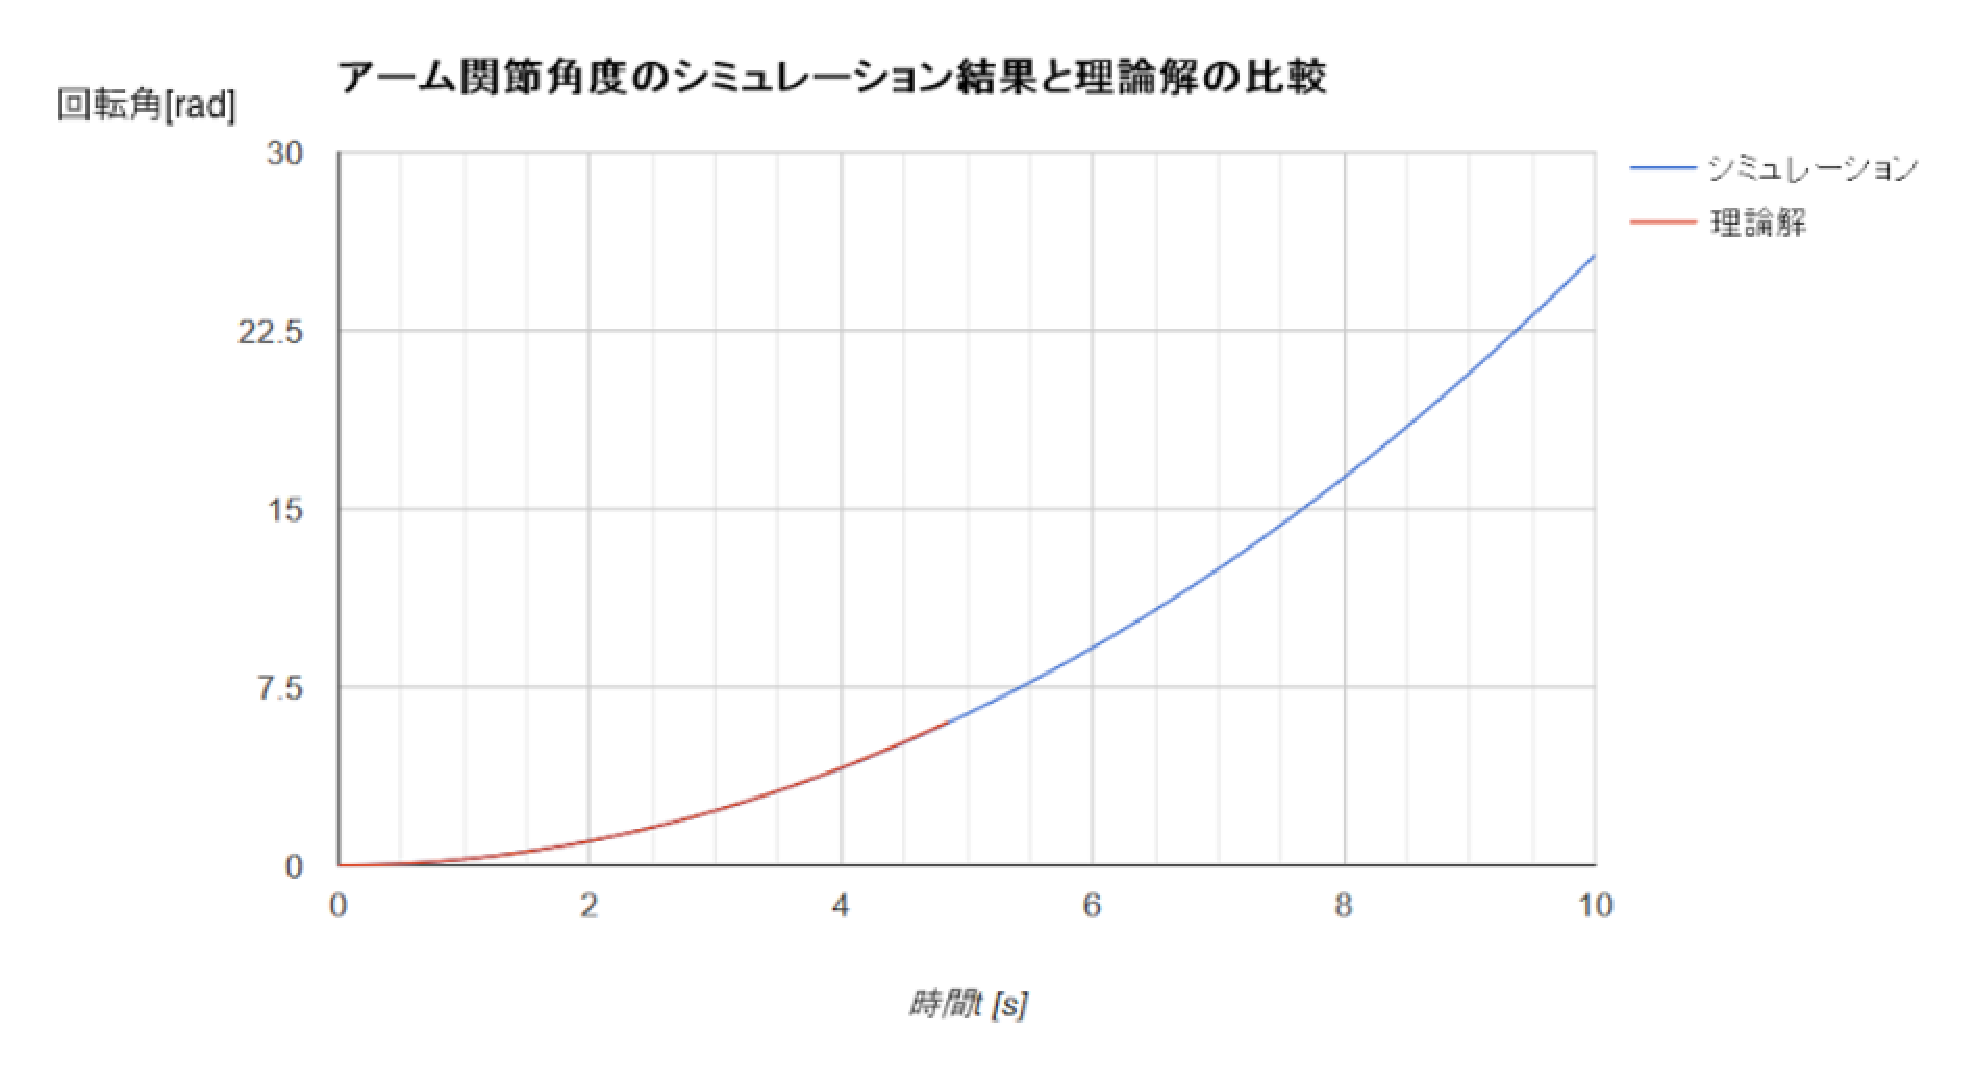
\includegraphics[height=7.5cm]{img/eps/strong-compare.eps}
    \end{tabular}
    \caption{シミュレーション結果と理論解の回転角度の比較}
    \label{strong-compare}
  \end{center}
\end{figure}

よって,このシミュレーション結果は正しいことが分かる.

手先加速度に関しては,基準ロボットの手先加速度について考えたときと同様に,手先速度のシミュレーション結果元にして手先加速度を割り出すという方法を取ることにする.

SimXpertより出力された手先速度を図\ref{strong-tesaki-sokudo}に示す.この時,青の破線が手先加速度のX方向成分,赤の破線が手先加速度のY方向成分,そして赤の実線が手先加速度のノルムを表している

\begin{figure}[htbp]
  \begin{center}
    \begin{tabular}{c}
      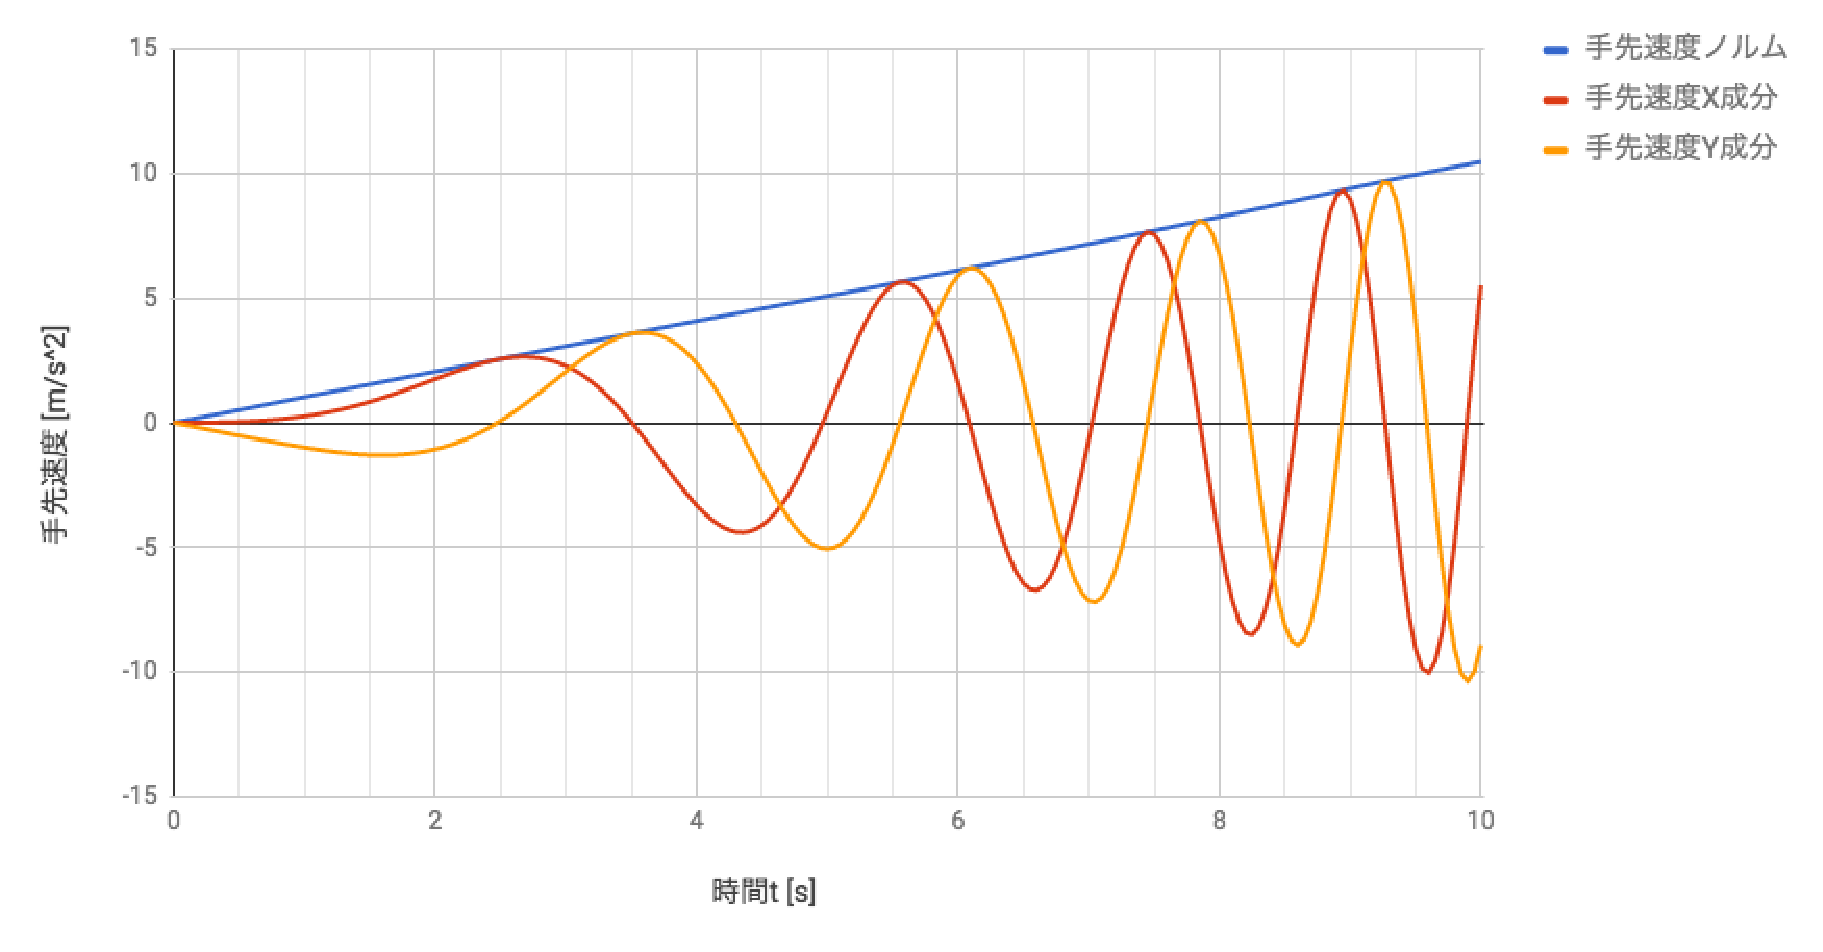
\includegraphics[height=5.5cm]{img/eps/strong-tesaki-sokudo2.eps}
    \end{tabular}
    \caption{手先速度のシミュレーション結果}
    \label{strong-tesaki-sokudo}
  \end{center}
\end{figure}

次に,この手先速度のシミュレーション結果の妥当性を理論解と比較することで検証する.

先ほど,式\ref{strong-niji-kinji}で,\(\theta = 0.2566t^2\)を得た.

角速度\(\frac{d\theta}{dt}\)は式\ref{strong-deg}を両辺\(t\)で時間微分することで得られるため,式\ref{strong-ddeg}となる.

\begin{eqnarray}
  \frac{d\theta}{dt} = 0.5132t
  \label{strong-ddeg}
\end{eqnarray}

ここで,角速度\(\frac{d\theta}{dt}\)と手先速度の大きさ\(v\)の間には,式\ref{strong-hand-vel}の関係がある.ただし,回転中心と手先間の距離を\(r\)と置いた.

\begin{eqnarray}
  v &=& r\frac{d\theta}{dt}
  \label{strong-hand-vel}
\end{eqnarray}

式\ref{strong-ddeg},及び式\ref{strong-hand-vel}より,手先速度の理論解の大きさは式\ref{strong-hand-velocity}となる.

\begin{eqnarray}
  v &=& r(0.5132t) \nonumber \\
    &=& 2(0.5132t) \nonumber \\
    &=& 1.0264t
  \label{strong-hand-velocity}
\end{eqnarray}

ゆえに,手先速度の理論解は\(v=1.0264t\)と求まった.

図\ref{strong-tesaki-sokudo}に示した,SimXpertによる手先速度のシミュレーション結果と,手先速度の理論解を比較したのが図\ref{strong-compare-vel}である.

\begin{figure}[htbp]
  \begin{center}
    \begin{tabular}{c}
      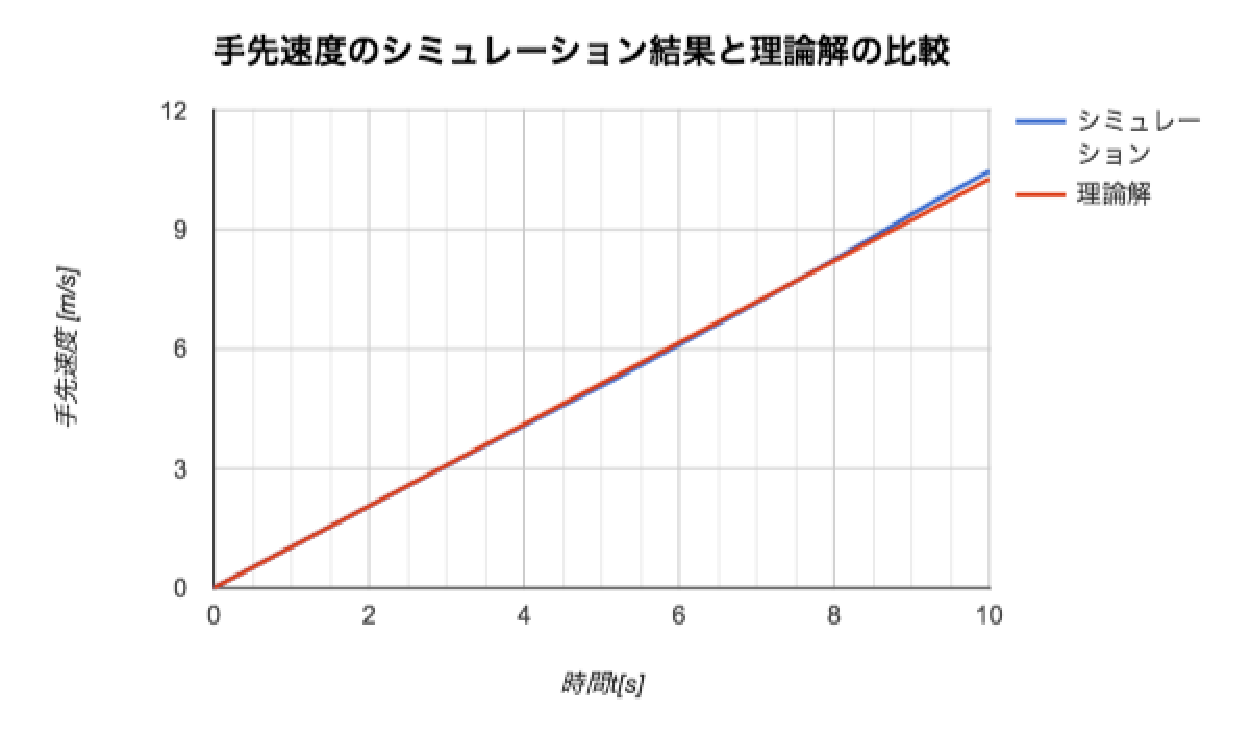
\includegraphics[height=8.5cm]{img/eps/strong-compare-vel.eps}
    \end{tabular}
    \caption{手先速度のシミュレーション結果と理論解の比較}
    \label{strong-compare-vel}
  \end{center}
\end{figure}

図\ref{strong-compare-vel}のグラフより,ほぼ完全に手先速度のシミュレーション結果と理論解は一致しているといえる.

SimXpertによって得られた手先速度のシミュレーション結果を最小二乗法によって1次関数近似を行うと,式\ref{strong-teaki-kinji}を得る.

\begin{eqnarray}
 v &=& 1.039t - 0.057 \nonumber \\
 &\approx& 1.038
  \label{strong-teaki-kinji}
\end{eqnarray}

手先速度のシミュレーション結果によって得られた式\ref{strong-teaki-kinji}と式\ref{strong-hand-velocity}の理論解は一致しており,シミュレーション結果が正しいと考えられる.

ここで,この手先速度を時間微分したものが手先加速度であるため,手先加速度として\(1.039[\rm m/s^2]\)を得る.

手先加速度の理論解および数値解のグラフを図\ref{strong-acc}に示す.

\begin{figure}[htbp]
  \begin{center}
    \begin{tabular}{c}
      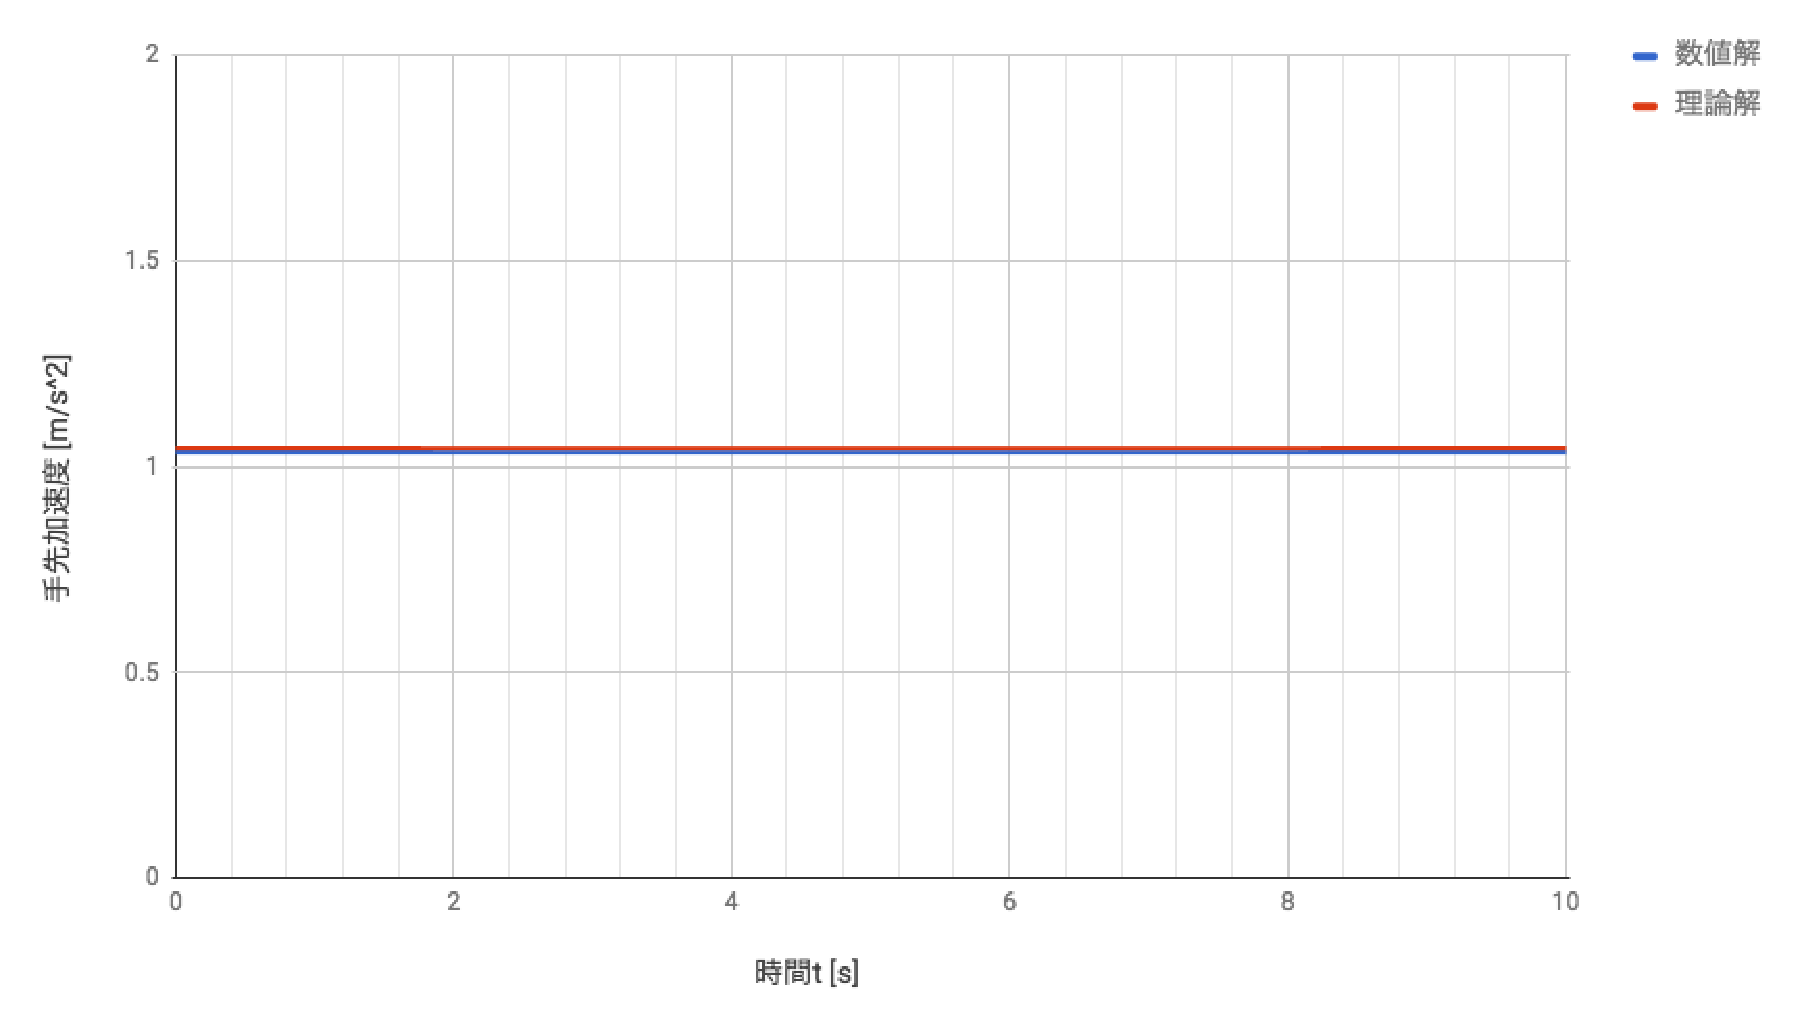
\includegraphics[height=5.5cm]{img/eps/strong-acc.eps}
    \end{tabular}
    \caption{手先加速度の理論解と数値解の比較}
    \label{strong-acc}
  \end{center}
\end{figure}
